% This is LLNCS.DEM the demonstration file of
% the LaTeX macro package from Springer-Verlag
% for Lecture Notes in Computer Science,
% version 2.4 for LaTeX2e as of 16. April 2010
%
\documentclass{llncs}
%
\usepackage{makeidx}  % allows for indexgeneration
\usepackage{graphicx}
\usepackage{subfigure}
\usepackage{color}
\graphicspath{{figs/}} 	
\usepackage{array}	
\usepackage{multirow}
		
	
%
\begin{document}
%
\frontmatter          % for the preliminaries
%
\pagestyle{headings}  % switches on printing of running heads
\addtocmark{Hamiltonian Mechanics} % additional mark in the TOC
%

%
\mainmatter              % start of the contributions
%
\title{ADHD-200 classification based on Social Network Method }
%
\titlerunning{Hamiltonian Mechanics}  % abbreviated title (for running head)
%                                     also used for the TOC unless
%                                     \toctitle is used
%
\author{Xiaojiao Guo\inst{1} \and Xiu An\inst{1}
 \and Deping Kuang\inst{1} \and Lianghua He\inst{1}}
%
\authorrunning{Ivar Ekeland et al.} % abbreviated author list (for running head)
%
%%%% list of authors for the TOC (use if author list has to be modified)
\tocauthor{Ivar Ekeland, Roger Temam, Jeffrey Dean, David Grove,
Craig Chambers, Kim B. Bruce, and Elisa Bertino}
%
\institute{The Key Laboratory of Embedded System and Service Computing, Ministry of Education,
Tongji University, Shanghai 201804, China
,\\
Department of Computer Science and Technology, Tongji University, Shanghai 201804, China,\\
\email{xiaojiaoguo12@gmail.com}}


\maketitle              % typeset the title of the contribution

\begin{abstract}
Attention Deficit Hyperactivity Disorder (ADHD) is one of the most common diseases in school aged children. In this study, we proposed a method based on social network to extract the features of the ADHD-200 resting state fMRI data between ADHD conditioned and control subjects. And the classification is done by using the support vector machine. The innovation of this paper lies in that: firstly, in the social network, the edge is defined by correlation between two voxels, where the threshold is proposed based on the optimal properties of small world; secondly, in the procedure of feature extraction, besides the traditional network features, we also exploit the new features such as assortative mixing and synchronization. We obtain an average accuracy of 63.75\%, which is better than the average best imaging-based diagnostic performance 61.54\% achieved in the ADHD-200 global competition. Compared with the proposed method, the result of the method based on traditional features is 61.04\% , which verified that the proposed method based on new features is better than traditional one.
\keywords{ADHD; fMRI; social network features; SVM}
\end{abstract}
%
\section{Introduction}
%
Attention Deficit Hyperactivity Disorder(ADHD), one of the most commonly found behavioral disorders, is characterized by inappropriate inattention and hyperactivity. Almost 5\% of school aged children are diagnosed with ADHD, which makes them difficult to control their behaviors or focus their attentions. And these behaviors may last for a particular length of time and result in impairment throughout their life\cite{1}. At present, the information that leads to this disorder is limited and the existing diagnoses rely largely on the physiopathologic symptoms. In fact, it is very difficult to classify the ADHD symptoms and normal by medicine clinical diagnoses accurately. Thus, there have great significance on the further studies on objective diagnosis of ADHD.


Functional magnetic resonance imaging (fMRI) is a widespread tool to measure brain activity in a non-invasive way in response to experimental conditions, because fMRI images obtained using blood oxygen level dependent (BOLD) contrast show signal fluctuations at rest. These fluctuations have been shown to be coherent across widely separated brain regions such as sensorimotor cortices\cite{2,3}. Studies have demonstrated ADHD related abnormalities in the interactions among brain regions supporting the implementation and maintenance of attention control by using resting state fMRI as an index of functional interactions\cite{4}. And we use the resting state brain fMRI data as   comparison to reflect the abnormalities in ADHD brains.


Recent advances in graph theoretical approaches have allowed us to characterize properties of brain networks. As one of the typical features of social network, the small world properties of brain networks are affected by normal aging and brain diseases\cite{5} such as Alzhermer's disease\cite{6}, epilepsy\cite{7} and schizophrenia\cite{8}. fMRI data can provide us the time-series of intensity values for each voxel, then the brain network can be constructed based on the correlation of the time-series. We choose social network features such as small world properties and degree of connectivity to discriminate the difference of ADHD and control brains fMRI data.


In this study, we use a large dataset from the ADHD-200 Global Competition challenged teams, which provides the large-scale resting state fMRI data of individuals with ADHD. Although there have lots of empirical studies, the clinical community still lack objective biomarkers to support the diagnosis and scientific community have not reached a comprehensive model of the disorder. The competition provides us an important opportunity to test fMRI data diagnosis for the reason that the ADHD-200 dataset collects data from 776 participants from multiple institutions contrast to that previous studies on fMRI-based diagnoses only included 39 participants on average\cite{9}. The details of the dataset and methods used in our study are explained in Section 2. The experimental results including the description of the experiment are presented in Section 3 and the conclusion from the experiment shows in Section 4.


\section{Materials and Methods}

%
\subsection{Dataset and Processing}
%
The data used in the present work is from the New York University Child Study Center (NYU) and Kennedy Krieger Institute (KKI) , which are part of the eight datasets of ADHD-200 Global Competition. Because the classification results on NYU dataset are the worst among ADHD-200 datasets at present, we choose it to compare with the average best results. NYU dataset contains a total number of 216 subjects including 118 ADHD whose age range from 7.17 to 17.61 (mean age 11.13) and 98 healthy controls whose age range from 7.17 to 17.96 (mean age 12.15). For processing, the resting state fMRI data are first subjected to a series of preprocessing steps, including 1) remove of a central spike caused by magnetic resonance signal offset, 2) slice timing,  3) 6-parameter rigid body motion correction to remove the head motions, 4) image registration to make image fuse between various imaging ways, 5) within-run intensity normalization to a whole brain mode value of 1000, 6) spatial smoothing with 8mm FWHM Gaussian kernel\cite{10}.


Then the Brodmann*s Interactive Atlas is applied to measure the functional connectivity among brain regions, which facilitates fMRI analysis understanding by providing access to all of the functions that have been associated with each of the Brodmann areas or corresponding gyri\cite{11}. The details of Brodmann areas for brain are provided in Fig. \ref{fig:1}. Now the resting state fMRI data of  Brodmann areas can be used to calculate and analysis properties by social network analysis. As known, social network analysis have been applied in various field such as mathematics, physics,information science, economics and scientific cooperation\cite{12}. As for brain network, few properties such as small world properties are used and we will apply other more features of better effects in this paper.


\begin{figure}[!htbp]
	\centering
		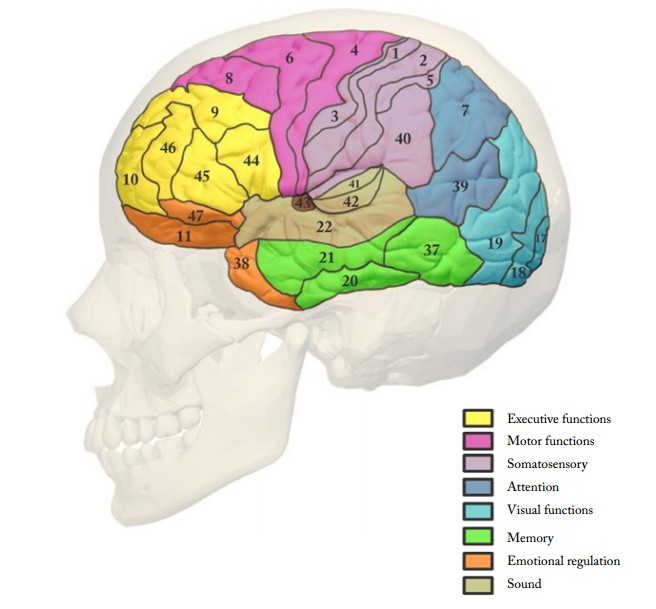
\includegraphics[scale=0.25]{figs/gxj1.jpg}
		\caption{Brodmann Cortical Areas}
    	\label{fig:1}
\end{figure}


\subsection{Network Construction}
fMRI data can be viewed as 4-D video so that the 3-D volumn of brain is divided into small voxels. The correlation of intensity time-series can be an indication of how synchronous the activities of two voxels are, and higher correlation values suggest that two voxels are working in synchronization. Symmetric correlation matrixes are produced by Pearson*s correlation coefficients between the time series of each possible pair of voxels of brain regions for each subject\cite{13}. Each correlation matrix is thresholded into a binary graph to investigate the properties of brain functional networks where nodes represent voxels of brain regions and edges represent undirected connections.


There is no definitive way currently to select a precise threshold in brain networks studies and the common way to explore the differences of network properties is to set threshold values on a wide range\cite{14,15}. In the present study, we use a new method to choose the proper threshold to obtain the most economical network. To diagnose small world properties, the characteristic path length and clustering coefficient were compared with the same metrics estimated in random networks configured with the same number of nodes, mean degree $K_{ran}$, and degree distribution as the network of interest, under the constraint that $K_{ran} > \log(n)$. Typically, in a small world network, we expect the ratio $\gamma =\frac{C_{net}}{C_{ran}}  >1$ and the ratio $\lambda = \frac{L_{net}}{K_{ran}} \approx 1$\cite{16,17}. Based on these, we select a threshold that makes $\gamma$ and $lamda$ optimal under the constraints at the same time, thus the most economical network can be constructed.


\subsection{Small World Properties}
Small world parameters of a network were originally proposed by Watts and Strogatz. The clustering coefficient $C_i (0 < C_i < 1)$ is a ratio that defines the proportion of possible connections that actually exist between the nearest neighbors of a node\cite{18}. The average of the clustering coefficients over all nodes $C_{net}$ quantifies the local inter-connectivity of a network and can be written
\begin{equation}
C_{net} = \frac{3 * number\;of\;triangles\; on\; the\; network}{number\; of\; connected\; triples\; of\; nodes}
\end{equation}

And high values of $C_i$ imply the most of nearest neighbors of that nodes are also nearest neighbors of each other or that node is located in a cliquish local neighborhood. The $L_{net}$ of a network is the mean of the $n-1$ minimum path lengths ($L_i$) between the index node and all other nodes in the network, where the minimum path length $L_i$ is the number of edges comprising the shortest path between any pair of nodes. $L_{net}$ is an indicator of overall routing efficiency of a network\cite{19}. To evaluate the small world properties, we generated 100 degree-matched random networks and scaled the $C_{net}$ and the $L_{net}$ of the real networks with the mean $\gamma$ (\ref{equ1}) and $\lambda$ (\ref{equ2}) of all the random networks\cite{20,21}. Typically, a small world network should fulfill the following conditions: $\gamma > 1$ and $\lambda \approx 1$\cite{17}. Therefore a scalar summary of small-worldness is that the ratio $\sigma = \gamma / \lambda$ is typically greater than 1\cite{22}. These conventional measures have been recently applied to many structural and functional brain networks studies\cite{5,6,23}.

\begin{equation}
\label{equ1}
\gamma = \frac{C_{net}}{C_{ran}}
\end{equation}

\begin{equation}
\label{equ2}
\lambda = \frac{L_{net}}{L_{ran}}
\end{equation}

\subsection{Assortative Mixing}
Assortative mixing is one of social network features and a network is said to show assortative mixing if the nodes in the network that have many connections tend to be connected to other nodes with many connections. Many networks show assortative mixing on their degrees, a preference for high degree nodes to attach to other high degree nodes while others show dis-assortative mixing that high degree nodes attach to low degree ones\cite{24}. Assortative mixing can have a substantial effect on the behavior of networked systems. Models that do not take it into account will necessarily fail to reproduce correctly many of the behaviors of real-world networked systems.


The networks that we might want to break up such as the social networks that spread disease, appear to be assortative and therefore are resilience, at least against simple targeted attacks such as attacks on the highest degree nodes. And yet at the same time the networks that we would wish to protect, including technological networks such as the Internet, appear to be dis-assortative and are hence particularly vulnerable\cite{25}. In this paper, we use the assortative mixing as one of the brain network features to distinguish the ADHD brains form controls. For the practical purpose of evaluating $r$ (assortative mixing) on an observed network,we can define as
\begin{equation}
r = \frac{M^{-1}\sum_ij_ik_i-[M^{-1}\sum_i\frac{1}{2}(j_i+k_i)]^2}
{M^{-1}\sum_i\frac{1}{2}(j_i^2+k_i^2)-[M^{-1}\sum_i\frac{1}{2}(j_i+k_i)]^2}
\end{equation}
Where $j_i$, $k_i$ are the degrees of the nodes at the ends of $i$th edge, with $i = 1,\cdots,M$.


\subsection{Other properties and the classification method}
Other properties of the social network are applied in the study, which may have better performance in the analysis. We quantify the dynamical implications of the small-world phenomenon by considering the generic synchronization of oscillator networks of arbitrary topology. The linear stability of the synchronous state is linked to an algebraic condition of Laplacian matrix of the network. The small world route produces synchronizability more efficiently than standard deterministic graphs, purely random graphs and ideal constructive schemes. However, the small world property does not guarantee synchronizability, the synchronization threshold lies within the boundaries, but linked to the end of the small world region\cite{26}. The synchronization is quantified by the ratio $S$ (\ref{equ3}) with $\lambda_2$ and $\lambda_N$ indicating the second smallest eigenvalue and the largest eigenvalue of the coupling matrix of the network, respectively.

\begin{equation}
\label{equ3}
S = \frac{\lambda_2}{\lambda_N}
\end{equation}



The hierarchical organization implies that small groups of nodes organize in a hierarchical manner into increasingly large groups while maintaining a scale-free topology. The degree of clustering characterizing the different groups follows a strict scaling law, which can be used to identity the presence of a hierarchical organization in real networks\cite{27}. And we define the hierarchical exponent $\beta$ as

\begin{equation}
C(k) \sim k^{-\beta}
\end{equation}


Support Vector Machine (SVM) can be characterized as a machine learning algorithm which maximizes the predictive accuracy without over-fitting the data to be trained and is capable of resolving linear and nonlinear classification problems. SVM works by mapping data to a high dimensional feature space and categorized, even when the data are not linearly separable. A separator between the categories is found and the data are then drawn into a hyperplane. Then, the characteristics of new data can be used to predict the group where a new record should belong. The boundary among the two categories can be defined by a hyperplane after the transformation. The kernel function of mathematical function is used in transformation. It supports the linear, Radial basis function (RBF) Polynomial and Sigmoid kernel types.


\section{Experimental Results}


The data preprocessing is applied to all resting state fMRI data from the ADHD-200 Global Competition, and the detailed steps have been described in Section 2. The preprocessed fMRI data that written into MNI space at 3 mm * 3 mm * 4 mm voxel resolution are divided into 48 regions according to the Brodmann areas. It is noneffective on some regions of 12, 13, 14, 15, 16, 31 and 33, for the data in these regions are empty. Then the network of each region is constructed by the correlation coefficient in the datasets of NYU and KKI. We calculate the properties of the social network such as small world properties and synchronization in each region network, and then train our SVM classifier with these properties. During the training and testing of SVM classifier, we used each subject in the dataset once as the validation data, and selected the optimal arguments by repeating this process the same times as the number of subjects with grid search algorithm. By a certain SVM training, we can obtain the average classification accuracy of 63.75\% and 78.21\% corresponding to NYU and KKI dataset respectively, which is better than the average best imaging-based diagnostic performance of 61.54\%, achieved in the ADHD-200 global competition\cite{28}. Particularly emphasized that, among the ADHD-200 global competition, NYU dataset achieves the lowest classification accuracy.
\begin{table}
\caption{The average accuracy based on different features}
\label{tab:1}
\begin{center}
\begin{tabular}{ccc}
\hline \rule{0pt}{12pt}
            	& \qquad\qquad NYU  \qquad\qquad   & \qquad\qquad KKI \qquad\qquad\\ [2pt]
\hline \rule{0pt}{12pt}
\quad All features	\quad & \qquad\qquad 0.6375 \qquad\qquad	&\qquad\qquad 0.7875 \qquad\qquad \\
\quad Small world properties	\quad& \qquad\qquad 0.6104 \qquad\qquad	&\qquad\qquad 0.7554 \qquad\qquad \\
\quad Others	\quad  & \qquad\qquad 0.6316 \qquad\qquad	&\qquad\qquad 0.7822 \qquad\qquad \\[2pt]
\hline
\end{tabular}
\end{center}
\end{table}




In order to make comparison, the classification has been performed in three ways to test the accuracy between the ADHD brain and controls, also to test the effect of social network features.  The three ways are respectively features of small world properties only, all features of social network analysis, and the other properties. The results of the average accuracy are shown in Table \ref{tab:1}. And the results of detailed region in three ways show in Fig. \ref{fig:2}. The best accuracies of the NYU and KKI dataset are 72.22\% and 85.71\%, separately appear in the region of 40 and 9.


\begin{figure}[!htbp]
	\centering
	\subfigure[]
    {
        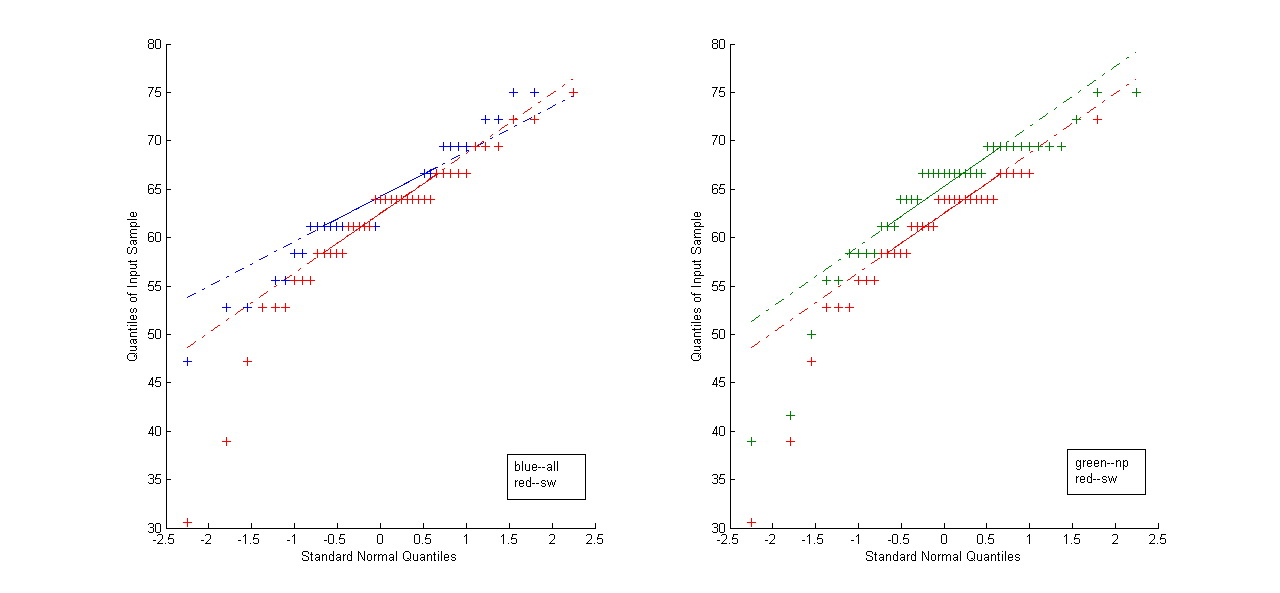
\includegraphics[scale=0.25]{figs/gxj2.jpg}
    }
    \\
    \subfigure[]
    {
        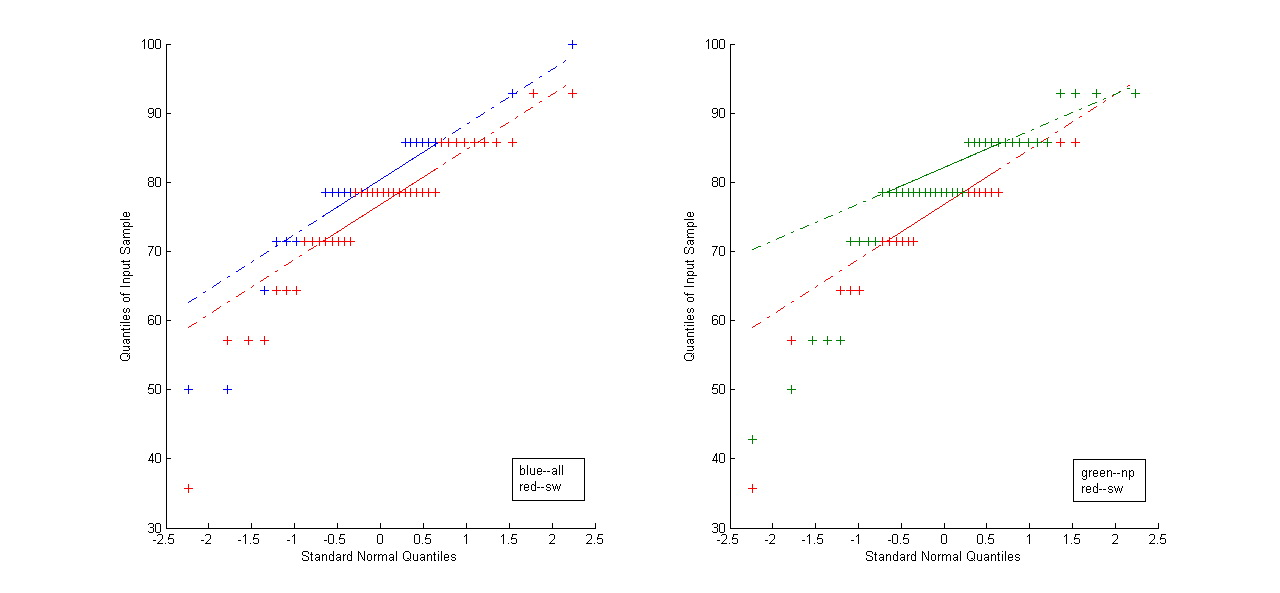
\includegraphics[scale=0.25]{figs/gxj3.jpg}
    }
	\caption{NYU and KKI experimental results}
    \label{fig:2}	
\begin{flushleft}
\emph{(a) shows the accuracy of detailed regions in three ways of NYU dataset. (b) shows the accuracy of detailed regions in three ways of KKI dataset. The blue indicates the accuracy of all features in classification while the red indicates the accuracy of small world properties used. On the right one, the green means the accuracy of the other features used in the classification.}
\end{flushleft}
    	
\end{figure}


Seen from Fig. \ref{fig:2}, we can find that the average accuracy among regions by using all features of social network is higher than that by only using small world properties. And also it can be seen that, there exists the same trend between the new features only and small world properties for both datasets, which in some degree verifies that the proposed method has a better effect than the one based on small world properties.



\section{Conclusion}
In this paper, a feature selection method based on social network analysis is applied, which can obviously reduce the computational complexity before SVM training. Nine kinds of features were extracted from the brain images and then used for training classifiers. It can be concluded from the experimental results that, the proposed method obtain a good performance of classification between ADHD diagnosed and control subjects. Also, we found that the features of assortative mixing and synchronization can be more effective in the classification than the traditional small world properties. The region of intermediate frontal, granular frontal and supramarginal gyrus corresponding to the area 8, 9 and 40, apparently have better performance in the classification, thus we have reason to consider that there exists obvious difference in these regions between ADHD and healthy subjects.


In the future work, we will verify the feasibility of the method for classification of other brain diseases, since we obtain a good result by applying the proposed method to classify between the ADHD diagnosis and controls in this paper. On the other hand, the classification accuracy may improve effectively if personal characteristic factor such as age, IQ etc. are also taken into account. And Future research will be needed to focus on this question.



%
% ---- Bibliography ----
%
\begin{thebibliography}{}
%
\bibitem{1}
Biederman,J., Mick, E., and Faraone,S. V.:
Age-dependent decline of symptoms of attention deficit hyperactivity disorder: impact of remission definition and symptom type.
Am. J. Psychiatry 157. 816每818 (2000)

\bibitem{2}
Biswal, B., Yetkin, F.Z., Haughton, V.M., Hyde, J.S.ㄩ
Functional connectivity in the motor cortex of resting human brain using echoplanar MRI.
J. Magn. Reson. Med 34. 537-541 (1995)

\bibitem{3}
Cordes, D., Haughton, V.M., Arfanakis, K., Wendt, G.J., Tursky, P.A.,Moritzk, C.H., Quigley, M.A., Meyerand, M.E.:
Mapping functionally related regions of brain with functional connectivity MR imaging.
AJNR Am. J. Neuroradiol 21. 1636-1644 (2000)

\bibitem{4}
Castellanos, F. X., Margulies, D. S., Kelly, C., Uddin, L. Q., Ghaffari, M.,Kirsch, A., Shaw, D., Shehzad, Z.,Di Martino, A., Biswal, B., SonugaBarke, E. J., Rotrosen, J., Adler,L. A., and Milham, M. P.:
Cingulate-precuneus interactions: a new locus of dysfunction in adult attention-deficit/hyperactivity disorder.
Biol. Psychiatry 63. 332每337 (2008)

\bibitem{5}
Achard S, Bullmore E:
Efficiency and cost of economical brain functional networks.
PLoS Comput Biol 3 e17. (2007)

\bibitem{6}
Stam C, Reijneveld J:
Graph theoretical analysis of complex networks in the brain.
Nonlin Biomed Phys. 1-3 (2007)

\bibitem{7}
Ponten SC, Bartolomei F, Stam CJ:
Small-world networks and epilepsy: Graph theoretical analysis of intracerebrally recorded mesial temporal lobe seizures.
Clin Neurophysiol 118. 918每927 (2007)

\bibitem{8}
Micheloyannis S, Pachou E, Stam CJ, Breakspear M, Bitsios P,Vourkas M, Erimaki S, Zervakis M:
Small-world networks and disturbed functional connectivity in schizophrenia.
Schizophr Res 87. 60每66 (2006)

\bibitem{9}
Shinkareva, S. V., Ombao, H. C., Sutton, B. P., Mohanty, A., and Miller, G. A.:
Classification of functional brain images with a spatio-temporal dissimilarity map.
Neuroimage 33. 63每71 (2006)

\bibitem{10}
Matthews P M, Jezzard P:
Functional magnetic resonance imaging[J].
Journal of Neurology, Neurosurgery \& Psychiatry 75(1). 6-12 (2004)

\bibitem{11}
Brauer J, Anwander A, Friederici A D:
Neuroanatomical prerequisites for language functions in the maturing brain[J].
Cerebral Cortex 21(2). 459-466 (2011)

\bibitem{12}
Sabater J, Sierra C:
Reputation and social network analysis in multi-agent systems[C].
Proceedings of the first international joint conference on Autonomous agents and multiagent systems: part 1, ACM. 475-482 2002

\bibitem{13}
Benjamini, Y. and Hochberg, Y.:
Controlling the false discovery rate: a practical and powerful approach to multiple testing.
Journal of the Royal Statistical Society, series B (Methodological). 289每300 (1995)

\bibitem{14}
Bullmore E, Sporns O:
The economy of brain network organization[J].
Nature Reviews Neuroscience 13(5). 336-349 (2012)

\bibitem{15}
Bassett DS, Meyer-Lindenberg A, Achard S, Duke T, Bullmore E:
Adaptive reconfiguration of fractal small-world human brain functional networks.
Proc Natl Acad Sci USA 103. 19518-19523 (2006)

\bibitem{16}
Watts DJ, Strogatz SH:
Collective dynamics of ※small-world§ networks.
Nature 393. 440每 442 (1998)

\bibitem{17}
Montoya JM, Sole RV:
Small world patterns in food webs.
J Theoret Biol 214. 405-412 (2002)

\bibitem{18}
Latora V, Marchiori M:
Efficient behavior of small-world networks[J].
Physical review letters 87(19). (2001)

\bibitem{19}
Newman MEJ:
The structure and function of complex networks.
SIAM Rev 45. 167-256 (2003)

\bibitem{20}
Maslov S, Sneppen K:
Specificity and stability in topology of protein networks.
Science 296. 910每913 (2002)

\bibitem{21}
Sporns O, Zwi JD:
The small world of the cerebral cortex.
Neuroinformatics 2. 145每162 (2004)

\bibitem{22}
Humphries MD, Gurney K, Prescott TJ:
Small world and scale-freeproperties of the brainstem reticular formation.
Proc R Soc Lond B Biol Sci. (2005)

\bibitem{23}
He Y, Chen ZJ, Evans AC:
Small-world anatomical networks in the human brain revealed by cortical thickness from MRI.
Cereb Cortex 17. 2407每2419 (2007)

\bibitem{24}
Newman M E J, Strogatz S H, Watts D J:
Random graphs with arbitrary degree distributions and their applications[J].
Physical Review E 64(2). (2001)

\bibitem{25}
Newman M E J:
Assortative mixing in networks[J]:
Physical review letters 89(20). (2002)

\bibitem{26}
Jespersen S, Sokolov I M, Blumen A:
Small-world Rouse networks as models of cross-linked polymers[J].
The Journal of Chemical Physics 113(17). 7652-7655 (2000)

\bibitem{27}
Gerdes S Y, Scholle M D, Campbell J W, et al.:
Experimental determination and system level analysis of essential genes in Escherichia coli MG1655[J].
Journal of bacteriology 185(19). 5673-5684 (2003)

\bibitem{28}
ADHD-200 global competition.
http://fcon\_1000.projects.nitrc.org/indi/adhd200. (2011)


\end{thebibliography}

\end{document}
